\documentclass[a4paper, notitlepage]{report}
\begin{titlepage}

\begin{center}

%% Insert the TU Delft logo at the bottom of the page.
\begin{tikzpicture}[remember picture,overlay]
    \node at (current page.south)[anchor=south,inner sep=0pt]{
        
\includegraphics{cover/logo}
    };
\end{tikzpicture}

%% Extra whitespace at the top.
\vspace*{2\bigskipamount}

%% Print the title in cyan.
{\makeatletter
\titlestyle\color{tudelft-cyan}\Huge\@title
\makeatother}

%% Print the optional subtitle in black.
{\makeatletter
\ifx\@subtitle\undefined\else
    \bigskip
    \titlefont\titleshape\LARGE\@subtitle
\fi
\makeatother}

\bigskip
\bigskip

by
%door

\bigskip
\bigskip

%% Print the name of the author.
{\makeatletter
\titlefont\Large\bfseries\@author
\makeatother}

\vfill

in partial fulfillment of the requirements for the degree of
%in overeenstemming met de vereisten voor het verkrijgen van de graad van

\bigskip
\bigskip

{\bfseries Master of Science}

in Applied Physics

\bigskip
\bigskip

at the Delft University of Technology,
%aan de Technische Universiteit Delft,

to be defended publicly on Tuesday January 1, 2013 at 10:00 AM.
%in het openbaar de verdedigen op dinsdag 1 januari om 10:00 uur.

\vfill

\begin{tabular}{lll}
%% Add additional information here, per faculty requirements, e.g
%    Student number: & 1234567 \\
%    Project duration: & \multicolumn{2}{l}{March 1, 2012 -- January 1, 2013} \\
    Supervisor: & Prof.\ dr.\ ir.\ A.\ Einstein \\
    Thesis committee:
        & Prof.\ dr.\ C.\ F.\ Xavier, & TU Delft \\
        & Dr.\ E.\ L.\ Brown, & TU Delft \\
        & Ir.\ M.\ Scott, & Acme Corporation
\end{tabular}

%% Only include the following lines if confidentiality is applicable.
\bigskip
\bigskip
\emph{This thesis is confidential and cannot be made public until December 31, 2013.}
%\emph{Op dit verslag is geheimhouding van toepassing tot en met 31 december 2013.}

\bigskip
\bigskip
An electronic version of this thesis is available at \url{http://repository.tudelft.nl/}.
%Een elektronische versie van dit verslag is beschikbaar op \url{http://repository.tudelft.nl/}.

\end{center}

\end{titlepage}


% All imports needed for file

% General
\usepackage[a4paper,top=1.25in,right=1in,bottom=1.25in,left=1in]{geometry}
\usepackage[utf8]{inputenc}
\usepackage[T1]{fontenc}
\usepackage{textcomp}
\usepackage[bitstream-charter]{mathdesign}
\usepackage{cite}

\usepackage{import}
\usepackage{standalone}
\usepackage{epstopdf}



% Math
\usepackage{amsmath}	% some standard math functions
%\usepackage{amssymb}	% more mathematical symbols
\usepackage{amsbsy}	% enable bold mathematics
\usepackage{bm}
%\usepackage{amsthm}	% enable theorem statements
\usepackage{trfsigns} 	% symbols for transforms

% Text formatting
\usepackage{fancyhdr}	% allow more control over page headers/footers
\usepackage{enumitem}	% allow control over enumerate, itemize, description
\usepackage{setspace}	% allow control over spacing
\usepackage{lastpage}	% provide label for last page in document
\usepackage{sectsty}	% allow control over section styling
\usepackage{url}

% Floats
\usepackage{xcolor}		% enable use of colors
\usepackage{graphicx}		% enable graphics
\usepackage{float}		% enable floats
\usepackage[section]{placeins}	% prevent floats from moving past e.g. sections
\usepackage[small, bf, hang, figurename=Fig.]{caption}	% enable captions for floats (images etc.)
\captionsetup{width=.8\textwidth} % captions not too wide
\usepackage{subcaption}		% enable subcaptions for floats (images etc.)
\usepackage[nottoc]{tocbibind}		% put more stuff in TOC

% Styling data
\pagestyle{fancyplain}

% Title page
\makeatletter
\let\inserttitle\@title
\makeatother

% Page header
\setlength{\headwidth}{\textwidth}
\lhead{} % leave left header empty
\chead{}
\rhead{} % leave right header empty
\lfoot{} % leave left footer empty
\cfoot{} % leave center footer empty
\rfoot{}
\renewcommand{\headrulewidth}{0.3pt}
\renewcommand{\footrulewidth}{0pt}

% Section, equation and figure numbering
\usepackage{chngcntr} 
\counterwithout{figure}{chapter}
\renewcommand{\thechapter}{\Roman{chapter}}
\renewcommand{\thesection}{\Roman{chapter}.\arabic{section}}
\renewcommand{\thesubsection}{\Roman{chapter}.\arabic{section}.\arabic{subsection}}
\renewcommand{\thesubsubsection}{\alph{subsubsection})}
\renewcommand{\thefigure}{\arabic{figure}}
\renewcommand{\thesubfigure}{\alph{subfigure}}
\renewcommand{\theequation}{\thechapter--\arabic{equation}}
\setcounter{tocdepth}{1}
\captionsetup[figure]{labelsep=period}

% Nice enumerations
\newlist{enum}{enumerate}{1}
\setlist[enum]{label=\textbf{[\arabic*]}} % \arabic or \alpha
\setlist{itemsep=-5pt}

% Nice \begin{StateDescription} for FSM descriptions
\newlist{StateDescription}{description}{1}
\setlist[StateDescription]{font=\normalfont\scshape, labelwidth=12em, leftmargin=12em,listparindent=0em,itemindent=0em}

% Section formatting
\definecolor{title-gray}{gray}{0.45}		% grijstint voor headers
\renewcommand*\sfdefault{lmss}
\allsectionsfont{\sffamily\color{title-gray}}	% sans-serif in headers

% Page layout
\onehalfspacing					% Wide margins for text
\usepackage{chngpage}			% customize margins of certain pages
\usepackage{adjustbox}

% Text macros
\usepackage{xspace}
\newcommand{\matlab}{MATLAB\xspace}		% fancy MATLAB command
\newcommand{\norm}[1]{\left\lVert#1\right\rVert}% Command for vector norm
\newcommand{\abs}[1]{\left\lvert#1\right\rvert}% Command for abs
\newcommand{\todo}[1]{\textbf{\textcolor{red}{#1}}}	% placeholder stuff
\let\oldhat\hat
\renewcommand{\vec}[1]{\bm{#1}} % bold vectors in math mode
\newcommand{\vechat}[1]{\oldhat{\bm{#1}}} % hat in vector mode
\newcommand{\mat}[1]{\bm{#1}} % bold matrix in math mode

%links
\usepackage{hyperref}
\hypersetup{ %setup hyperlinks
    colorlinks=true,
    citecolor=black,
    filecolor=black,
    linkcolor=black,
    urlcolor=black
}

\begin{document}

\section{System performance}
\subsection{Android}
Despite the lack of real-time guarantees from the Android kernel and the overhead inherent to Java applications, no performance problems were encountered in the Android data acquisition application.

Unfortunately, the Android \texttt{AudioRecord} API does not make adequate provisions for querying the supported audio recording settings for a given device. The suggested way of determining whether a given mode is supported is to attempt to initialize using these settings, and catching any thrown exceptions as well as detecting whether the resulting object was successfully initialized. Unfortunately, this process is unreliable, and it was found that while testing, certain phones successfully initialized the AudioRecord object but e.g. yielded duplicated mono data when a stereo signal was requested, or yielded corrupted data.

In addition, which processing is performed for each configurable audio source varies per device. Certain devices turn on specialized signal processing that negatively affects the beamforming processing, such as automatic gain control or noise reduction algorithms. Android unfortunately lacks an adequate API for requesting audio sources with a certain amount of processing performed or querying the processing performed for each audio source. Experimentation showed the voice recognition input (\texttt{AudioSource.VOICE\_RECOGNITION}) generally yielded the least amount of processing, but even this was not guaranteed in all cases.

\subsection{Server application}
Although no attempt was made to quantify the performance of the server application, it can be said that no problems were encountered with the server application, with up to 6 simultaneous phones streaming their audio recordings at once. Furthermore, all packets described in section \ref{subsec:communication-protocol} are correctly encoded, decoded and interpreted. The orientation measurements are passed on to a function translating them into azimuth and elevation estimates. Recorded audio data is passed on to a buffer structure used in the beamforming system \cite{BAP:ErikNiels}.

\paragraph*{}
One feature of the server implementation is that it does not use any functions specific to \matlab or Java (e.g. functions that are not available in other common programming languages). This ensures the application may be ported to a different programming language, although performance was found to be adequate for the purposes of this system. A major advantage of using \matlab was the ease of interfacing with the beamforming subsystem, which also runs in \matlab \cite{BAP:ErikNiels}.

For a future, more fully-fledged product, the use of \matlab should be reconsidered. Performance issues might arise when more complex operations are performed simultaneously with the server application, and the interface between \matlab and Java that was used is not officially supported.

\section{Orientation measurement}
\label{sec:orientation_measurement}
As the beamforming algorithm relies on directivity data that varies with the orientation of the phone, it is necessary to determine the orientation of each smartphone. As no research was found detailing the accuracy of smartphone orientation sensors on a table in an office environment, it was deemed necessary to characterize the accuracy of the orientation sensors in the smartphones in this situation.

The experimental setup is shown in Fig.~\ref{fig:orientation_measurement_setup}. A table was set up in an office environment. Three smartphones were placed in three locations on the table, two of which were located above the metal leg assembly of the table. For each location, the smartphones were placed in the same orientation by aligning them with the edges of the table. Every second, the orientation of each phone was computed based on its internal sensors, in the manner described in section \ref{sec:android}. Next, this data was transmitted to a computer running the server application described in section \ref{sec:matlab}. This orientation was logged for 30 minutes per run, after which the phones were switched to another of the three locations. The experiment was repeated three times to acquire data for each phone in each position.

Representative results for the computed azimuth are shown in Fig.~\ref{fig:orientation_az_loc1}. The reported azimuths are reasonably constant over the measurement interval but individual computed azimuths already vary by over 20 degrees. Full results may be found in Fig.~\ref{app:orientation_total} in the appendix. A discussion of the results may be found in section \ref{sec:disc_orient}.

\begin{figure}[htb]
\centering
\end{figure}

\begin{figure}[H]
\begin{adjustwidth}{-1in}{-1in}
\centering
	\begin{subfigure}{0.5\textwidth}
		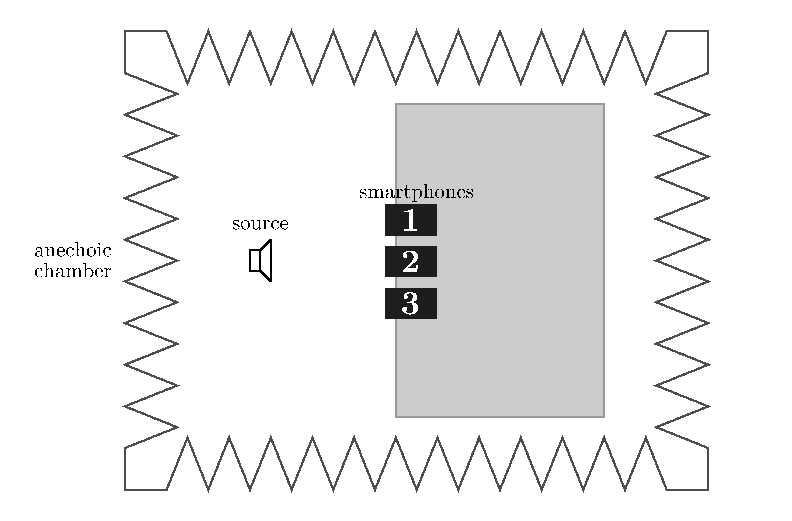
\includegraphics[width=\textwidth]{figures/orientation/measurement_setup}
		\caption[Measurement setup used for orientation measurements.]{Schematic representation of the measurement setup used for orientation measurements. The figure shows the top view of a table with measurement locations indicated by the numbers. The grey area indicates the location of metal support bars of the table.}
		\label{fig:orientation_measurement_setup}
	\end{subfigure}
	\begin{subfigure}{0.5\textwidth}
		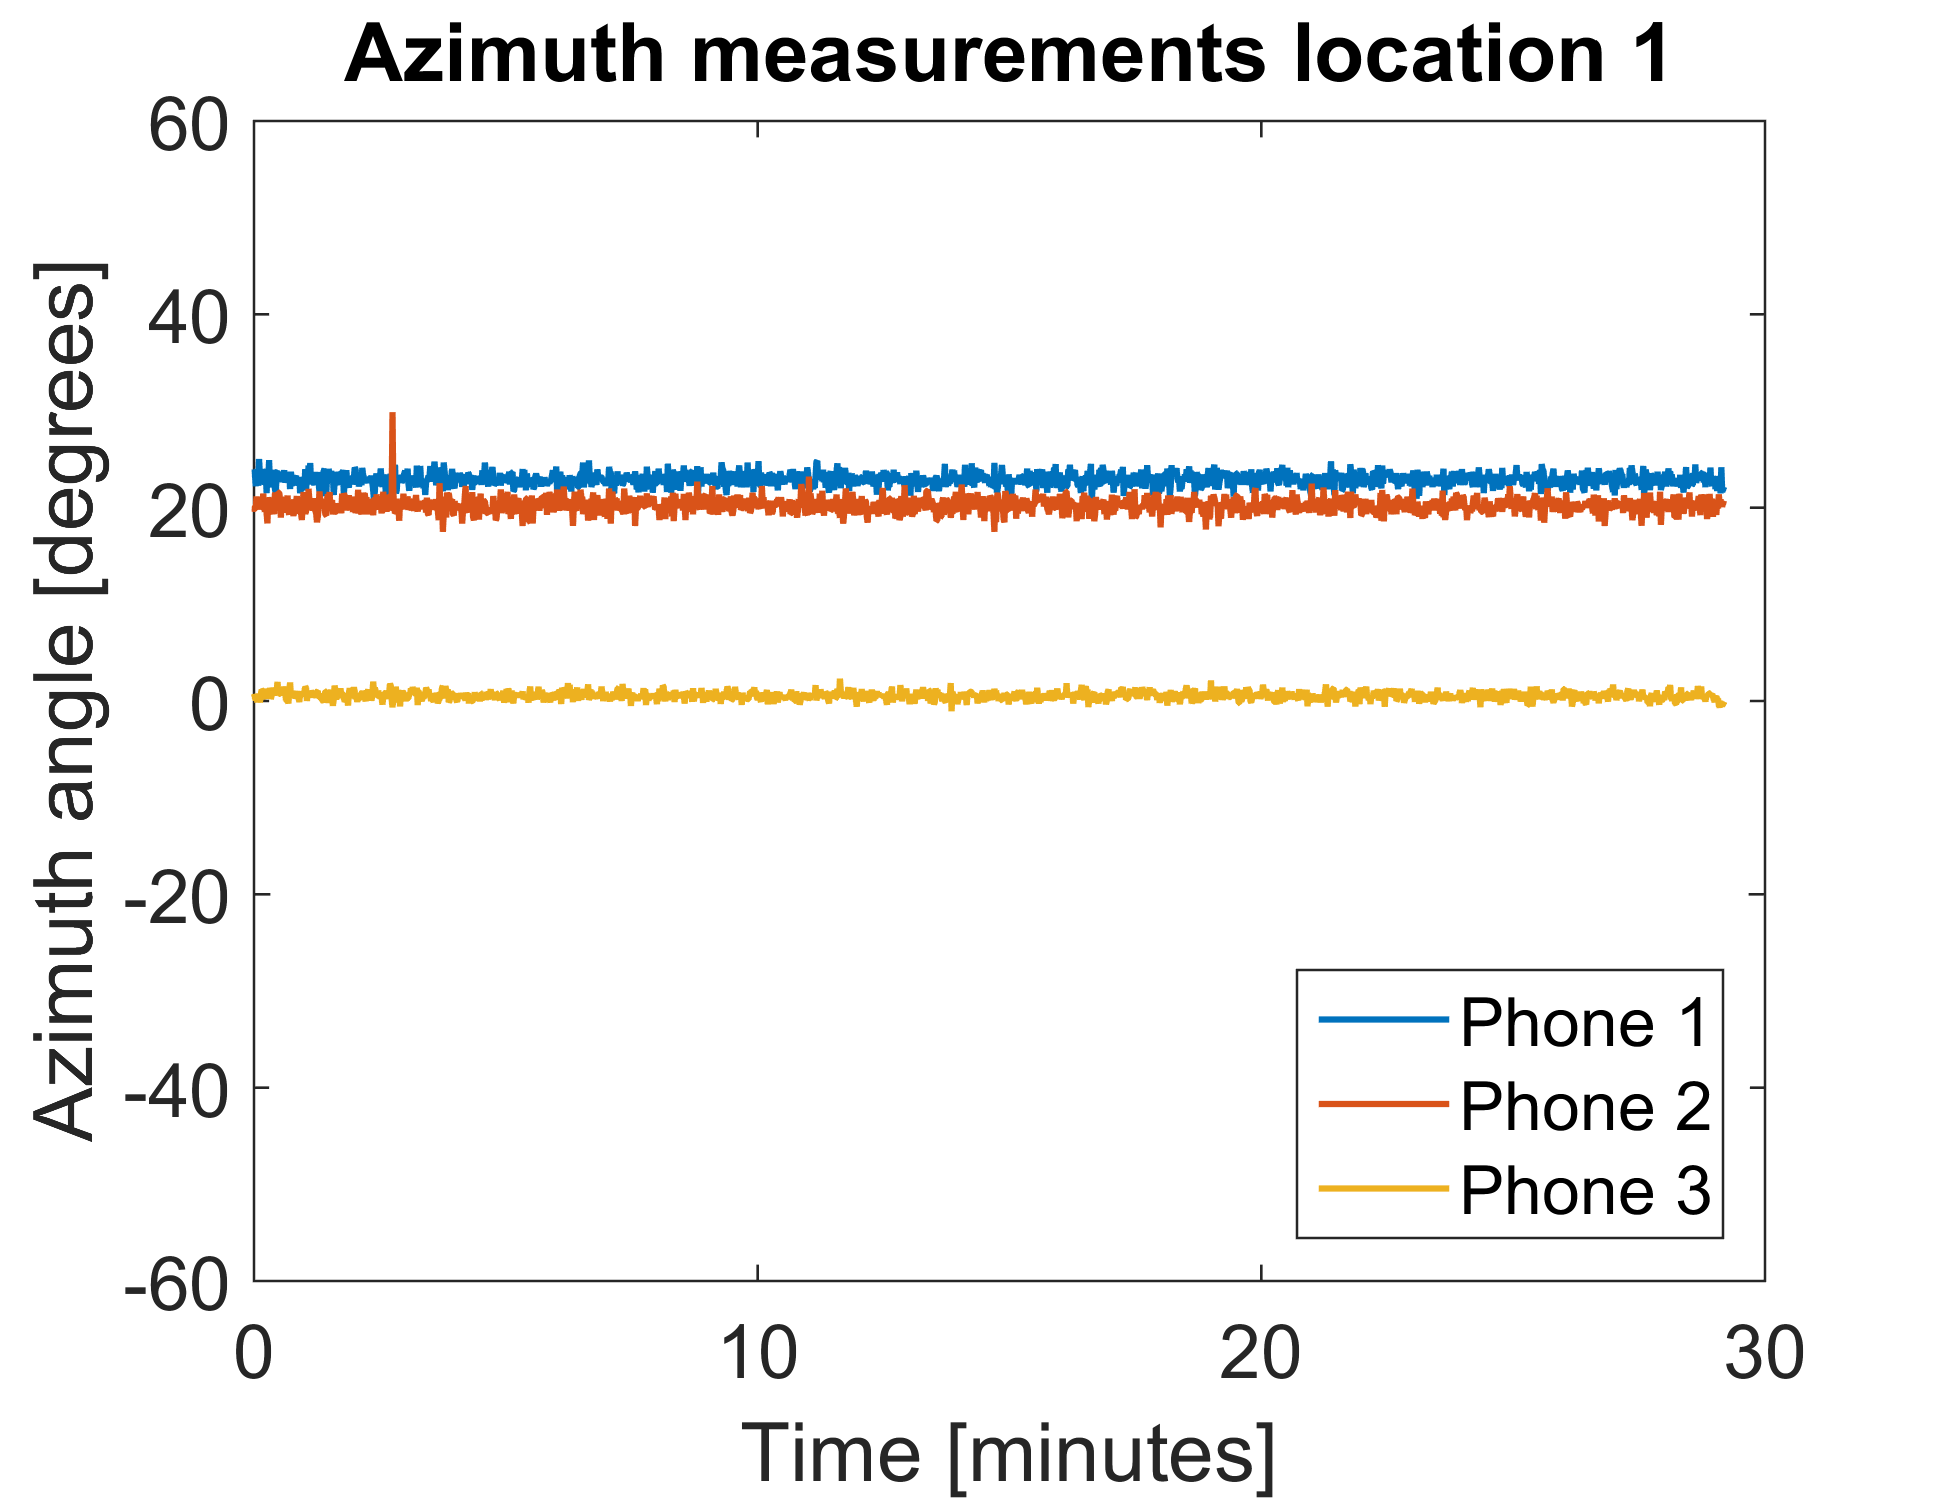
\includegraphics[width=\textwidth]{figures/orientation/az_loc1}
		\caption{Azimuth angles for location 1.}
		\label{fig:orientation_az_loc1}
	\end{subfigure}
\end{adjustwidth}
\caption[Measurement of smartphone orientations.]{Measurement setup for orientation estimation and azimuth angles from three smartphones. The azimuth is quite constant, but a large offset is present between different sensor readings at the same location. Full results for all smartphones and locations can be found in Fig.~\ref{app:orientation_total} in the appendix.}
\label{fig:orientation}
\end{figure}

\end{document}
